% IMPORTANT: PLEASE USE XeLaTeX FOR TYPESETTING
\documentclass{sintefbeamer}
\usepackage{xeCJK}
\usepackage{amsthm}
\setbeamertemplate{theorems}[numbered]
\makeatletter
\setbeamertemplate{footline}
{
  \leavevmode%
  \hbox{%
  \begin{beamercolorbox}[wd=.7\paperwidth,ht=2.25ex,dp=1ex,center]{title in head/foot}%
    \usebeamerfont{title in head/foot} {GFL: Federated Learning on Non-IID data via Privacy-preserving Synthetic data}
  \end{beamercolorbox}%
  \begin{beamercolorbox}[wd=.3\paperwidth,ht=2.25ex,dp=1ex,right]{date in head/foot}%
    \usebeamerfont{date in head/foot}\insertshortdate{}\hspace*{2em}
    \insertframenumber{} / \inserttotalframenumber\hspace*{2ex} 
  \end{beamercolorbox}}%
  \vskip0pt%
}

%\newtheorem{theorem}{Theorem} % to number according to section
\theoremstyle{definition}

\makeatother

% meta-data
\title{\huge GFL: Federated Learning on Non-IID Data via Privacy-preserving Synthetic Data}
\subtitle{汇报人:黄其涵 \qquad 导师:章静 教授 \qquad }
\author{2023 IEEE International Conference on Pervasive Computing and Communications (PerCom)}
\date{\today}
\titlebackground{images/bg4}

% document body
\begin{document}

\maketitle


\section{研究背景}

\begin{frame}{1.1 联邦学习}
\begin{itemize}
\item 联邦学习是一种分布式机器学习方法,其利用一个中央服务器(也称为服务器端)协调各终端设备(也称为客户端),协同训练一个各客户端共享的全局模型。

\item 与传统中心化训练方法不同,\textbf{联邦学习不需要各设备发送自身隐私数据至数据中心,因此有利于保护数据隐私。}具体而言,联邦学习在客户端和服务器端之间通过多轮通信迭代优化模型。
\item 每轮通信包含两个阶段:
\begin{itemize}
\item[(1)]各客户端从服务器端下载全局模型,并在本地数据上进行训练以获得本地模型;
\item[(2)]服务器端接收并聚合各客户端的本地模型参数以获得性能更优的全局模型.然而,现有联邦学习机制尚面临两大不足。
\end{itemize}
\end{itemize}

\end{frame}

\begin{frame}{1.1 联邦学习}
\begin{itemize}
\item 联邦学习是一种分布式机器学习方法,其利用一个中央服务器(也称为服务器端)协调各终端设备(也称为客户端),协同训练一个各客户端共享的全局模型。

\item 与传统中心化训练方法不同,\textbf{联邦学习不需要各设备发送自身隐私数据至数据中心,因此有利于保护数据隐私。}具体而言,联邦学习在客户端和服务器端之间通过多轮通信迭代优化模型。
\item 每轮通信包含两个阶段:
\begin{itemize}
\item[(1)]各客户端从服务器端下载全局模型,并在本地数据上进行训练以获得本地模型;
\item[(2)]服务器端接收并聚合各客户端的本地模型参数以获得性能更优的全局模型.然而,现有联邦学习机制尚面临两大不足。
\end{itemize}
\end{itemize}

\end{frame}

\begin{frame}{1.2 现有问题}
\begin{columns}
\begin{column}{0.45\textwidth}
\begin{figure}[ht]
\centering
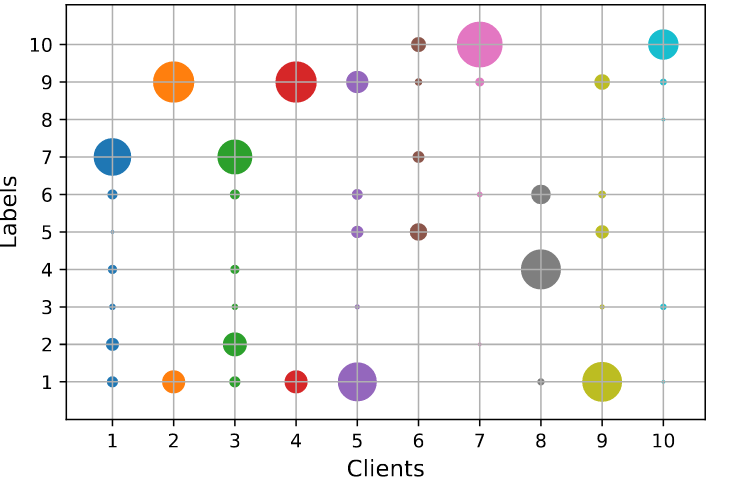
\includegraphics[width=1\textwidth]{images/img_unbalance}
\end{figure}
\end{column}
\begin{column}{0.65\textwidth}
\begin{itemize}
\item \textbf{类别不均衡。}全局模型需考虑多个客户端的数据,但各客户端往往仅包含部分类别数据且类别间数据量严重不均衡,使得全局模型难以训练。所训练的本地模型容易过拟合本地数据而在全局数据上往往取得较差性能。更重要的是,这些性能较差的本地模型严重影响全局模型的训练,导致难以构建高性能全局模型。
\item \textbf{数据分布差异。}由于各客户端的功能和用户使用习惯不同,不同客户端往往产生不同类别的数据,导致各客户端数据之间的类别分布差异较大。
\end{itemize}
\end{column}
\end{columns}
\end{frame}


\begin{frame}{1.3 主要贡献}
\begin{itemize}
\item \textbf{本文提出基于GAN的GFL框架以解决FL中数据异构性问题,并为 FL 系统构建高性能全局模型。 }GFL 促进了 FL 训练过程,同时保持了成员身份的隐私和原始数据在客户中的分布。
\item \textbf{本文提出了一种保护隐私的数据生成工作流程,以生成符合我们隐私设置的合成样本。} DPGAN 用于生成满足差分隐私的样本,以保护客户端免受成员推理攻击。本文生成大量合成数据并选择一个随机分布的子集来隐藏客户端的真实数据分布。
\item \textbf{本文对合成数据进行“iidify”处理,以 iid 方式训练全局模型,并使用 Epoch Decay 参数来解决模式崩溃问题并避免使用低质量的合成数据。}
\end{itemize}
\end{frame}

\section{问题定义}

\begin{frame}{2 优化目标}

\begin{columns}
\begin{column}{0.4\textwidth}
\begin{figure}[ht]
\centering
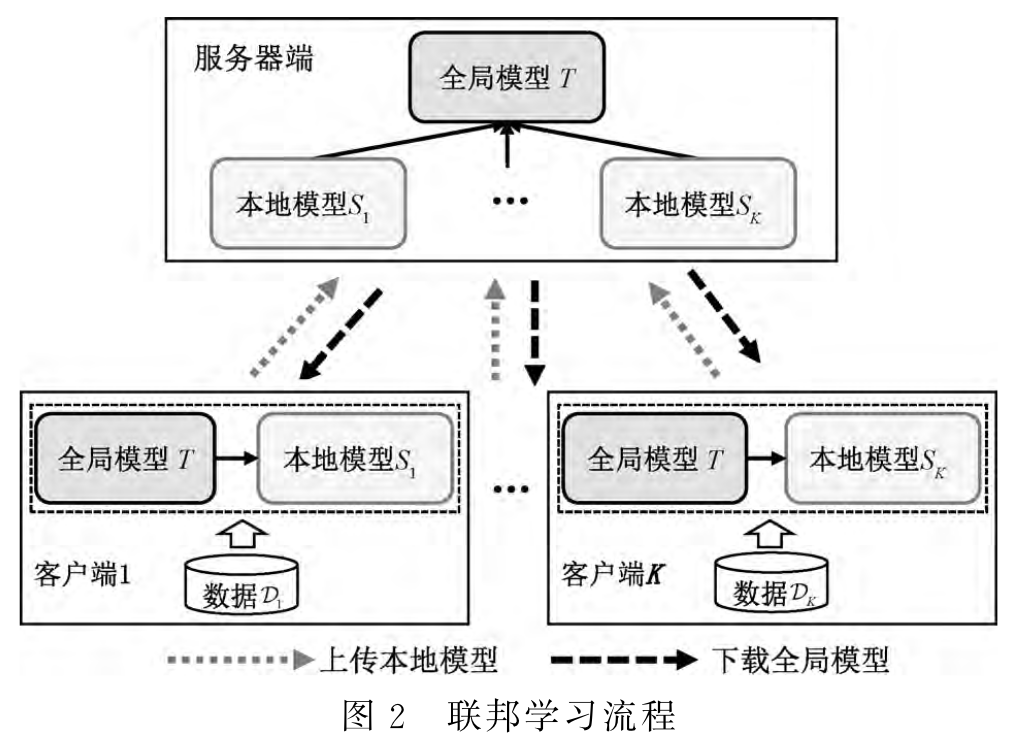
\includegraphics[width=1\textwidth]{images/img_fl}
\end{figure}
\end{column}
\begin{column}{0.6\textwidth}
为解决上述难题, 本文提出在客户端构造类别均衡的数据集进行训练的策略。 令 $\mathcal{D}$ 表示所构造的类别 均衡数 据集, $M$ 表示全局数据的类别数,则 
$$
\mathcal{D}=\left\{(x, y) \mid P(y=i)=\frac{1}{M}, \quad i \in\{0,1, \ldots, M-1\}\right\}
$$
其中 $p(\mathcal{D})$ 表示数据集 $\mathcal{D}$ 所代表的经验分布. 因此, 本文 旨在解决如下优化问题:
$$
\min _{\boldsymbol{W}_T} \mathbb{E}_k\left[\mathbb{E}_{x_k \sim p(\mathcal{D})}\left[\mathcal{L}\left(x_k ; \boldsymbol{W}_T\right)\right]\right]
$$
与仅仅利用客户端本地数据进行训练的方式相比,基于类别均衡的数据集进行训练使得各客户端本地模型之间的差异大大减少。
\end{column}
\end{columns}


\end{frame}

\section{研究方法}

\begin{frame}{3.1  Overview of Generative Federated Learning (GFL)}
\centering
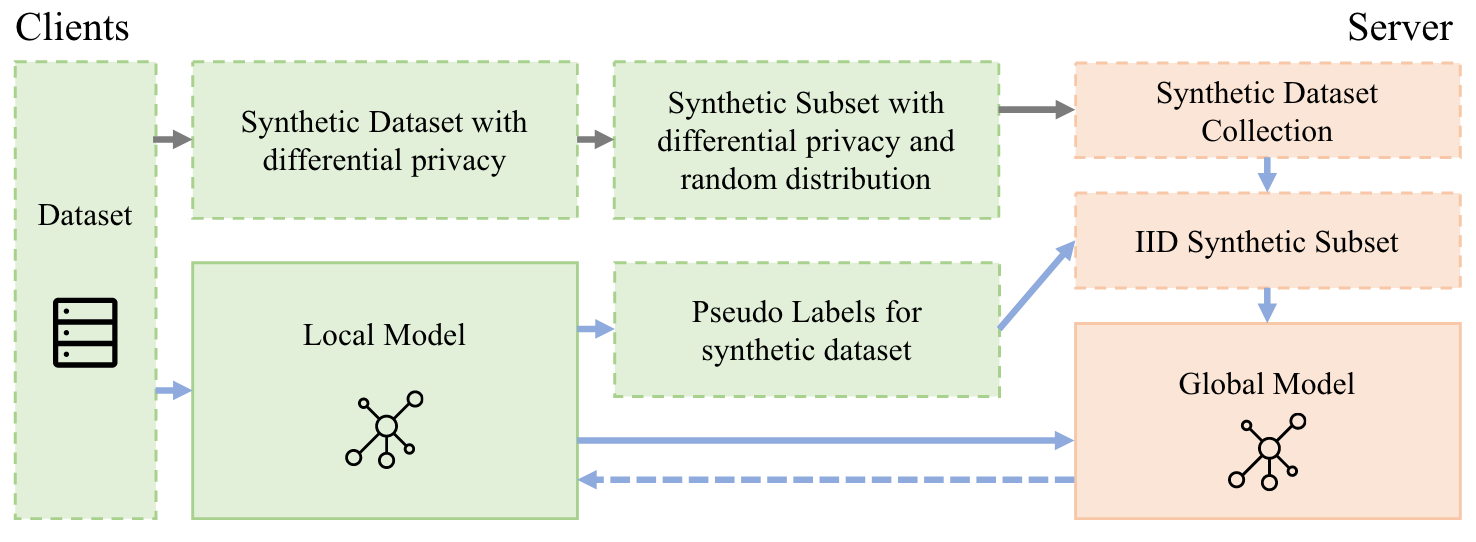
\includegraphics[width=1\textwidth]{images/gfl_overview}

\end{frame}

	
\begin{frame}{3.2 Synthetic Data Generation}{Threat Model}
	将 GAN 引入 GFL 中的联邦学习。但是,GAN 提供的合成数据可能会泄露客户的隐私信息。 \textbf{GAN 中最严重的漏洞之一是成员关系问题。例如,即使他/她参加了 GAN 训练,也没有人希望他/她的脸出现在生成的图像中。}
		\\ \hspace*{\fill} \\
	本文将考虑虚拟一个对手(GFL中的服务器),他的目的是\textbf{推断一个单一的已知记录是否包括在受害者(目标GAN模型)的训练集中,这被称为成员推理攻击。}对手是半诚实的,他遵循正常的训练过程,但对成员关系很好奇。作为对手的半诚实服务器处于如下所述的黑盒设置中。

\begin{itemize}
\item The architecture of the victim.
\item The parameters and training hyper-parameters of the victim.
\item The dataset used in the victim.
\end{itemize}

\end{frame}

\begin{frame}{3.2 Synthetic Data Generation}{Privacy-preserving Data Generation}
\textbf{服务器作为协调整个 FL 训练的角色,本文希望它能够主动参与训练,而不是被动地聚合参数。}由于缺少特征信息,我们想为服务器创建一个小型 iid 数据集,以帮助在短时间内找到全局最优值。这个 iid 数据集中的数据应该完全来自客户端,所以仍然面临着共享时数据隐私信息可能泄露的挑战。
\\ \hspace*{\fill} \\
本文专注于抵抗成员推理攻击和防止数据分布信息泄漏,在合成数据生成阶段,提供了一种实现合成数据隐私保护生成的解决方案。


\end{frame}



\begin{frame}{3.2 Synthetic Data Generation}{Privacy-preserving Data Generation}


\begin{columns}
\begin{column}{0.5\textwidth}
\begin{figure}[ht]
\centering
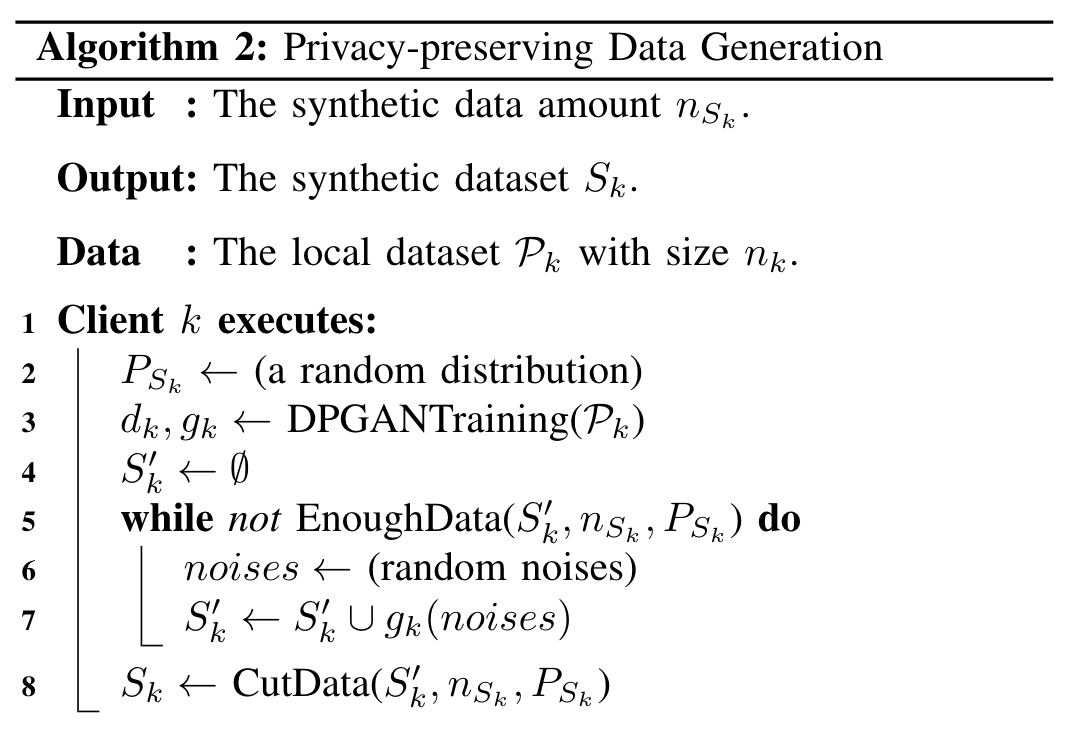
\includegraphics[width=1\textwidth]{images/algo2_1}
\end{figure}

\end{column}
\begin{column}{0.5\textwidth}
\begin{figure}[ht]
\centering
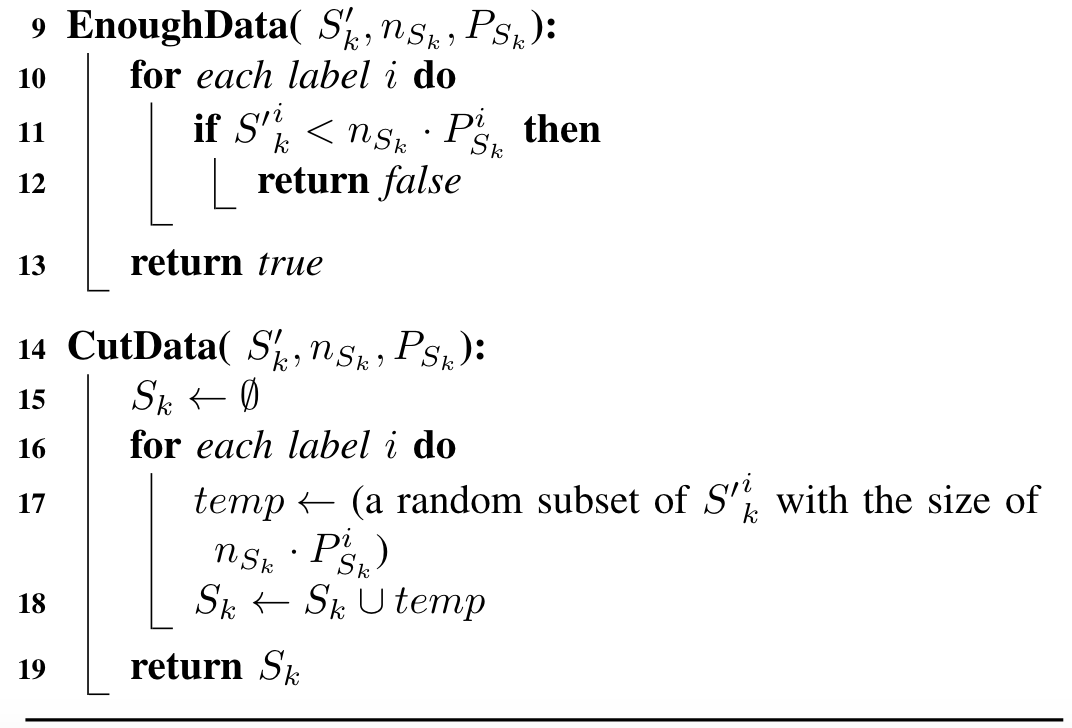
\includegraphics[width=1\textwidth]{images/algo2_2}
\end{figure}
\end{column}
\end{columns}


\end{frame}


\begin{frame}{3.3 Federated Learning with Synthetic Data}
\begin{columns}
\begin{column}{0.4\textwidth}
\begin{figure}[ht]
\centering
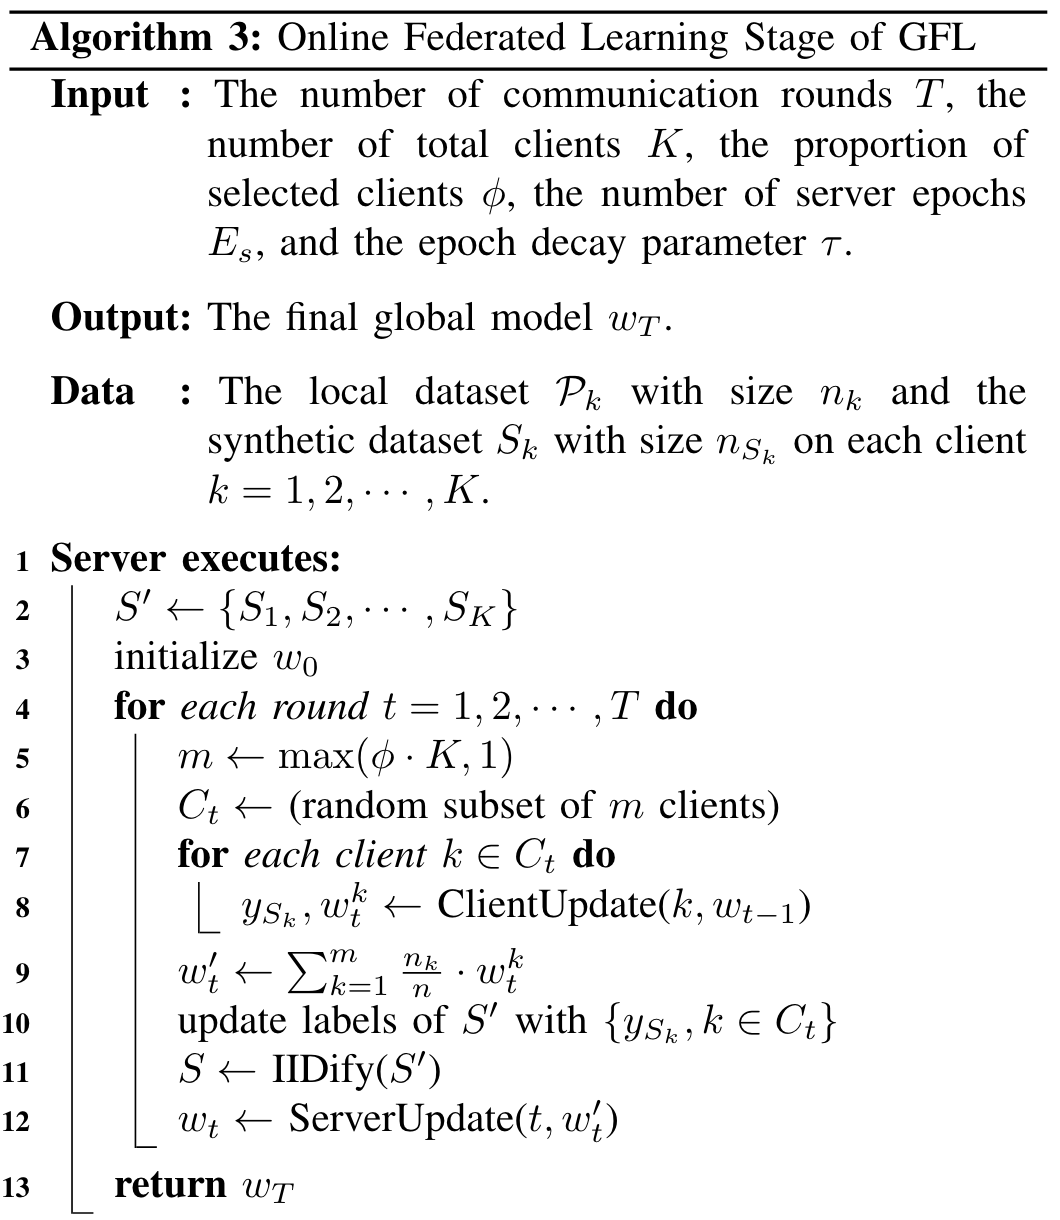
\includegraphics[width=1\textwidth]{images/algo3_1}
\end{figure}

\end{column}
\begin{column}{0.4\textwidth}
\begin{figure}[ht]
\centering
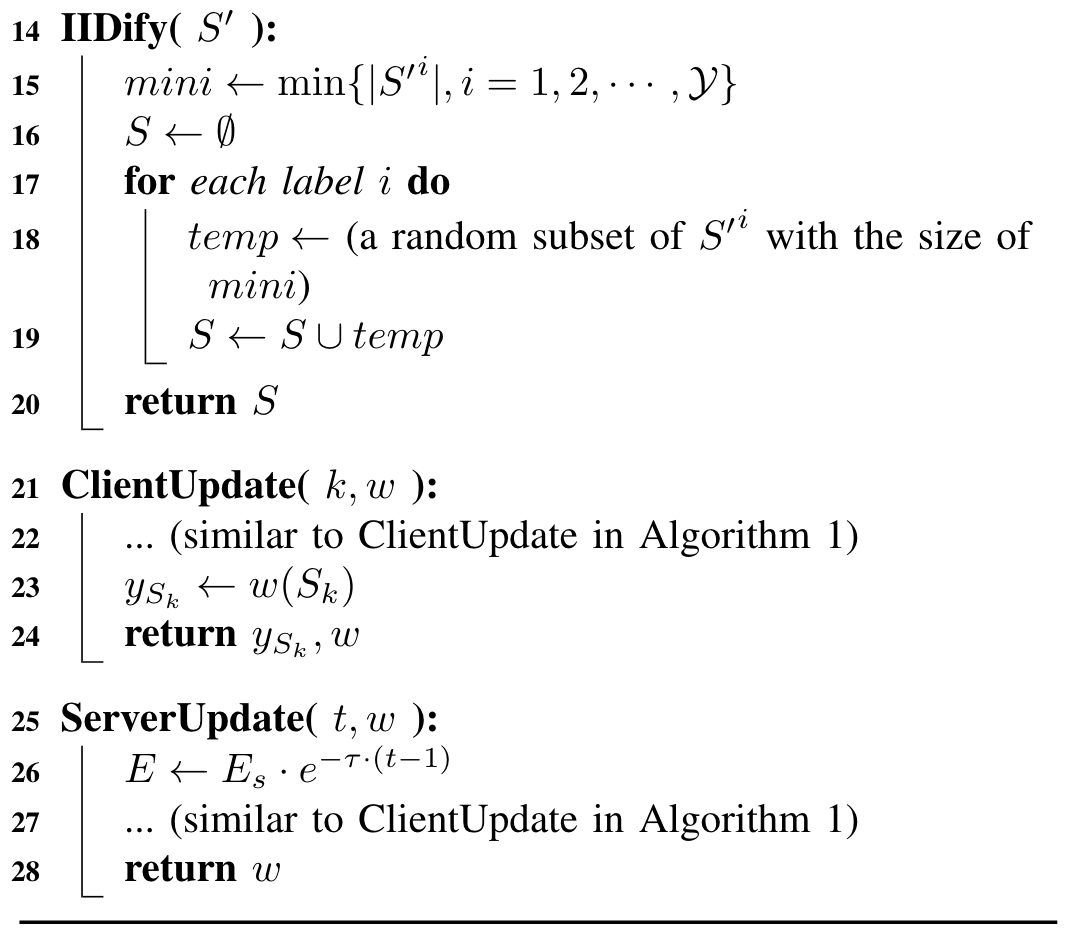
\includegraphics[width=1\textwidth]{images/algo3_2}
\end{figure}
\end{column}
\end{columns}
\end{frame}





\section{实验分析}

\begin{frame}{4.1 数据配置}{数据集}

在我们的实验中,我们使用 DPGAN 作为Local GAN模型,ResNet18 作为 EMNIST 和 CIFAR-10联邦学习的训练模型。

	\begin{itemize}
\item[1)] EMNIST。 在实验中使用它的“Digits”子集。它包含 10 个类,总共 280, 000 个样本,分为 240, 000 个训练样本和 40, 000 个测试样本。与 MNIST 相比,它拥有更多数据并且完全平衡。
\item[2)] CIFAR-10。它包含 10 个不同类别的 60, 000 个 32 × 32 彩色图像,与 EMNIST 相比,这是一项更复杂的任务。我们使用这个数据集来衡量 GFL 在艰巨任务中的稳定性。
\end{itemize}
\end{frame}

\begin{frame}{4.2 数据配置}{Dirichlet Distribution}
\begin{figure}[ht]
\centering
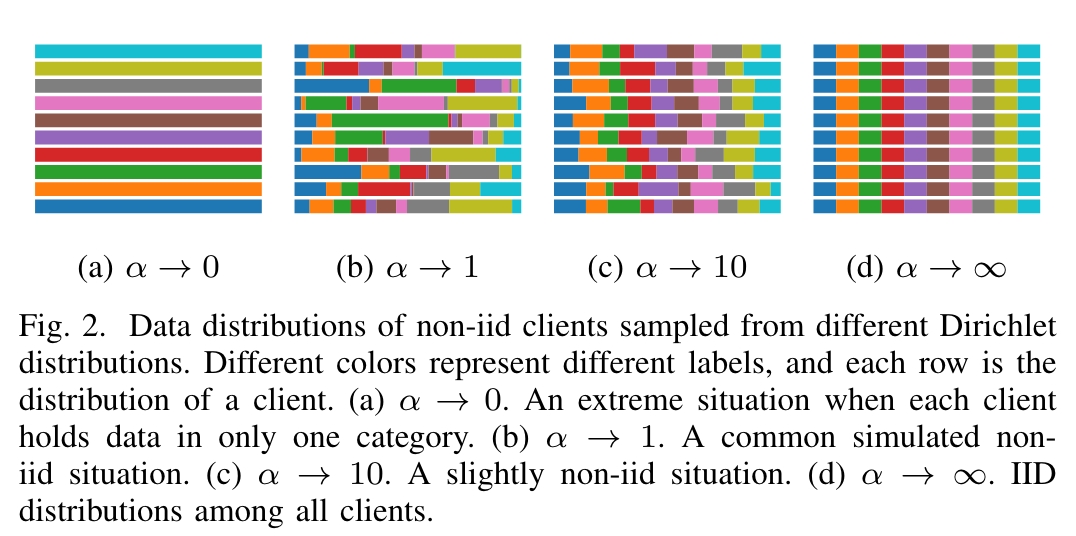
\includegraphics[width=0.85\textwidth]{images/dir}
\end{figure}
\end{frame}


\begin{frame}{4.2 对比模型}
本文将GFL与目前最新的方法进行比较,即FedAvg、FedPoxr、SCAFFOLD和FedNvao。本实验通过狄利克雷分布Dir(0.1)模拟各客户端数据的类别分布。
	\\ \hspace*{\fill} \\
GFL 在合成数据生成阶段训练了 200 个 epoch。然后,我们从每个客户端 $k$ 中随机选择 $n_{S_k}=500$  个合成样本。在联邦学习阶段,初始全局训练 epoch $E_s$ 设置为 10,如果未指定,epoch decay 参数 $\tau$ 设置为 0.1。
	\\ \hspace*{\fill} \\
上述所有算法共享相同的基本训练设置。训练包含 100 轮通信,每轮每个客户端训练 20 个 epoch,服务器和客户端的批大小都设置为 128。
\end{frame}


\begin{frame}{4.3 实验结果}{Result Analysis}
\begin{figure}[ht]
\centering
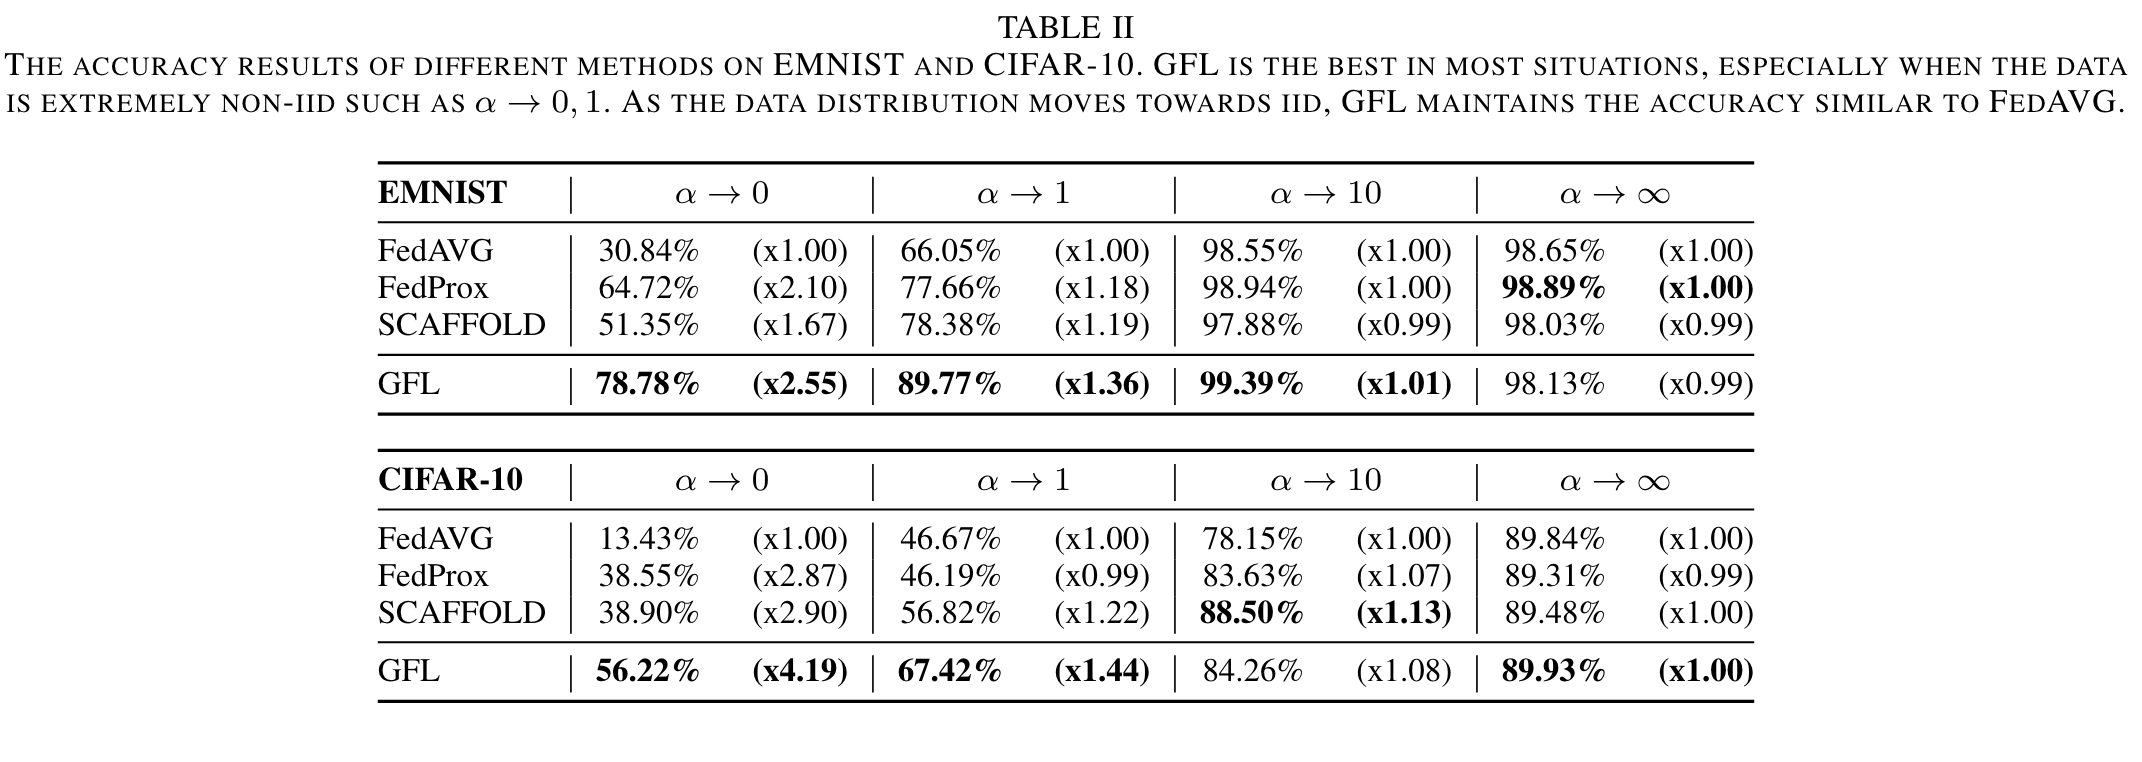
\includegraphics[width=1.\textwidth]{images/res_table2}
\end{figure}
	1. GFL 在所有设置中都优于其他算法; 2. non-iid程度越大,GFL的优势越明显; 3.数据集越复杂,GFL 越优越。
\end{frame}

\begin{frame}{4.3 实验结果}{Result Analysis}

\begin{figure}[ht]
\centering
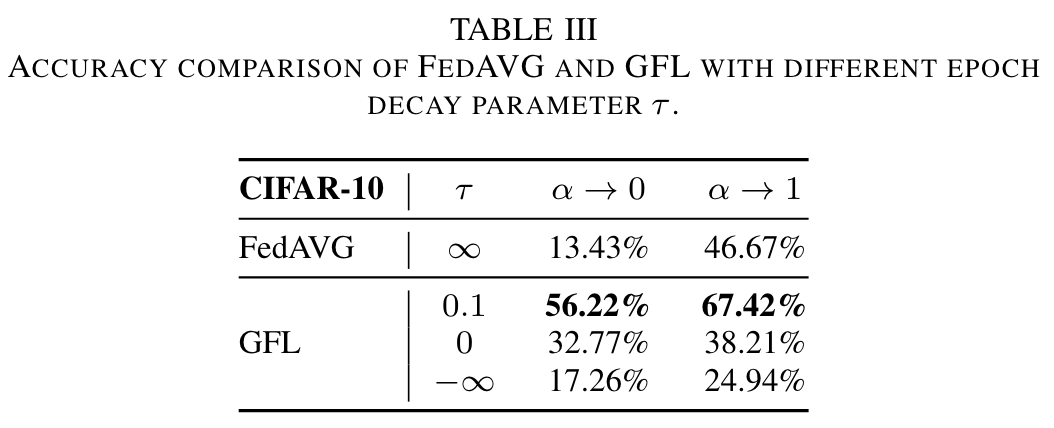
\includegraphics[width=0.75\textwidth]{images/res_table3}
\end{figure}
	
	1. Epoch Delay参数在 GFL 中是必不可少的;
	 
	2. 只使用合成数据的方法是没有用的。
\end{frame}

\begin{frame}{4.3 实验结果}{Result Analysis}

\begin{figure}[ht]
\centering
	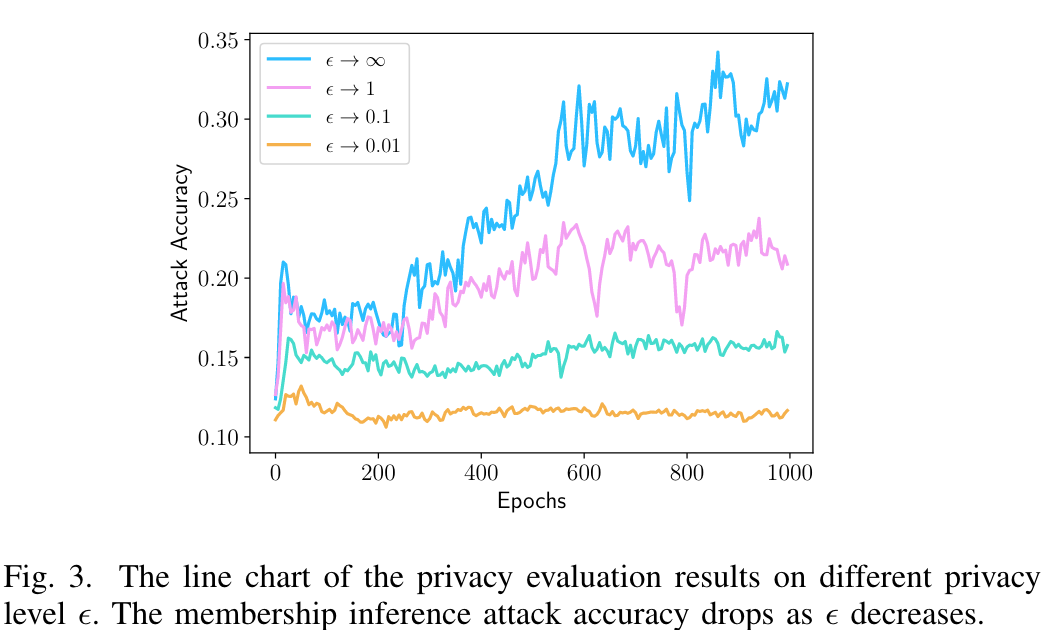
\includegraphics[width=0.75\textwidth]{images/res_fig3}
	\end{figure}
\end{frame}


\begin{frame}{4.3 实验结果}{Result Analysis}
\begin{figure}[ht]
\centering
	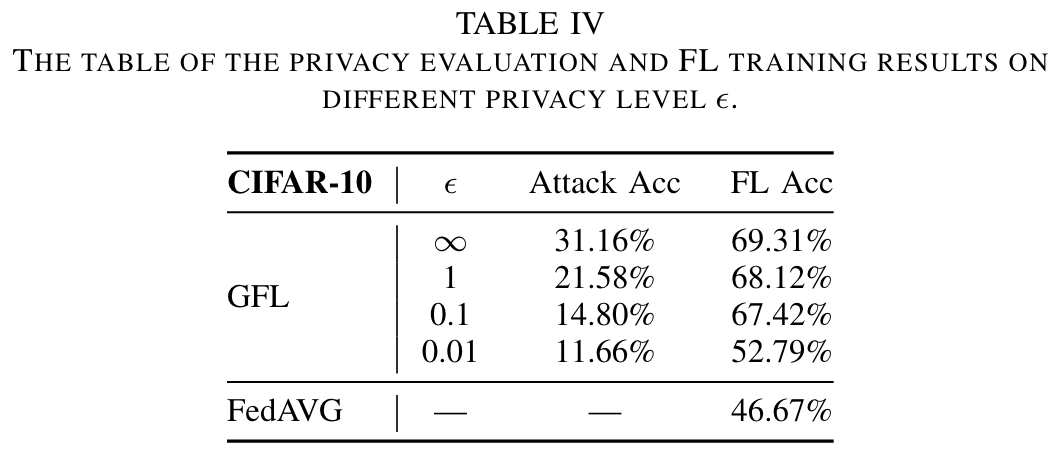
\includegraphics[width=0.75\textwidth]{images/res_table4}
	\end{figure}
	
	根据图 3 和表 IV 中的实验,选择$\epsilon$ = 0.1,这可以防止成员推理攻击,同时保持良好的性能。
\end{frame}



\section{研究总结}

\begin{frame}{研究总结}

本文提出了一个称为生成联合学习 (GFL) 的新框架来处理非独立同分布问题。我们将 DPGAN 引入 GFL 以应对潜在的隐私攻击,尤其是成员推理攻击。
\\ \hspace*{\fill} \\
大量实验表明,GFL 可以在非 iid 情况下工作,也可以在 iid 情况下工作,并且在大多数情况下优于其他框架,如 FedProx 和 SCAFFOLD。隐私评估表明,通过在 DPGAN 的训练中加入适当的噪声,我们可以有效地防御成员推理攻击。我们还分析了 GFL 引入的Epoch Decay 参数的必要性,这对于防止模式崩溃和低质量样本损害全局模型很重要。


\end{frame}



\backmatter

\end{document}
